\documentclass{article}

\usepackage[margin=100pt]{geometry}

\usepackage[UTF8]{ctex}
\usepackage{longtable}

\graphicspath{ {images/} }


\begin{document}

\title{进度汇报}
\author{易亚洲 U201315168}

\maketitle

\section{提交内容(2月23日)}

\begin{enumerate}
	\item 进度安排
	\item 系统的主要模块
	\item 主要的功能描述
\end{enumerate}


\section{进度安排}

项目的工作主要安排在2017年2月13日至2017年5月22日。相关重要时间点如下:
\begin{enumerate}
	\item 开题,第四周前(2017年3月10日前)
	\item 中期检查,第九周前(2017年4月10日前)
	\item 完成论文编写,第15周前(2017年5月22日前)
	\item 答辩和验收,第18周前(2017年6月16日前)
\end{enumerate}

具体时间及任务安排如下:

\begin{longtable}[h!]{|c|l|l|}
\caption{研究进度安排表}
\\\hline
周次 	& 日期 & 任务安排\\\hline
1		& 2.13~2.19 & 收集相关文献,了解Android安全和防火墙的最新研究,编写文献综述\\\hline
2		& 2.20~2.26 & 体验和研究现有的防火墙应用,进行市场调查\\\hline
3		& 2.27~3.5  & 完成需求分析,确定方案可行性,了解项目要求的技术知识\\\hline
4		& 3.6 ~3.10 & 完成开题报告\\\hline
5		& 3.11~3.19 & 完成好相关准备工作,进行总体模块划分,确定各模块的总体设计\\\hline
6,7		& 3.20~4.2  & 编码实现,完成核心功能\\\hline
8,9 	& 4.3 ~4.16 & 编码实现图形界面\\\hline
10		& 4.17~4.23 & 进行基本功能的测试\\\hline
11,12	& 4.24~5.7  & 增加更多功能,完善兼容性,性能优化和改善易用性\\\hline
13 		& 5.8 ~5.14 & 进行完整的功能测试,兼容性测试和性能测试\\\hline
14 		& 5.15~5.22 & 对开发工作进行整理,编写论文报告\\\hline
\end{longtable}


\section{模块设计}

根据实现防火墙的原理和功能需求,设计了成如图的应用架构。

\begin{figure}[!h]
\centering
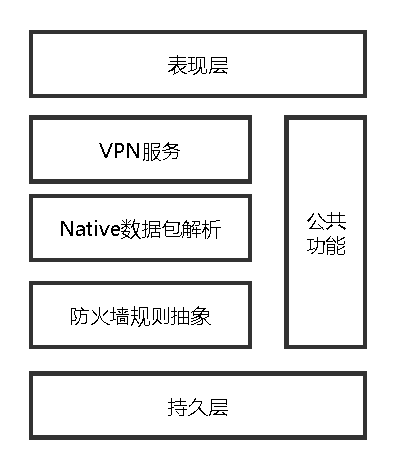
\includegraphics[width=.6\textwidth]{modules.pdf}
\caption{应用模块层次}\label{fig:5}
\end{figure}

\begin{itemize}
	\item 表现层\\ 表现层采用Activity作为主要实现,为用户提供友好的图形界面,是用户操作和管理防火墙的门户,是所有功能的入口,同时也承担着,在VPN服务层返回相应的信息(比如要求用户对是否允许某个应用的连接进行选择)时,对用户进行提醒;
	\item VPN服务模块\\该模块是继承并实现Android提供的VpnService的关键组件,用以实现VPN的功能,将VPN过滤的流量传递到下一层进行解析,并根据解析和匹配的结果,向系统回应是否作相应的处理;
	\item Native数据包解析模块\\该层主要完成将网络数据包进行解析,从中提取协议、地址、会话时间等关键信息,并用防火墙规则进行匹配,判断数据包是否放行;
	\item 防火墙规则抽象模块\\该模块负责管理持久层的防火墙规则数据,将持久层信息抽象成相应的Java对象,供Native数据包解析模块使用;同时,由于在大量数据包中,规则的读取极其频繁,防火墙规则抽象模块也负责实现对规则的缓存,提高性能;
	\item 持久层\\主要负责为上层模块提供持久化储存,主要包括SQLite数据库和SharePreference存储:防火墙规则采用关系型数据库进行储存,而其他公共功能的信息采用SharePreference储存;
	\item 公共功能\\除核心防火墙之外的功能,如用户向导,版本更新,配置导入导出等功能由于功能简单,不在划分更加详细的模块层次。
\end{itemize}




\section{功能设计}

用户期望一个Android防火墙应用提供友好的交互界面和正常的拦截效果。设计中应实现:
\begin{itemize}
    \item 拦截管理界面:对某个应用设置是否拦截流量
    \item 全局控制开关:切换全局防火墙状态
    \item 查看历史通信日志:查看单个应用的通信日志,包括尝试访问的地址,端口,协议类型,
    \item 设置亮屏等特殊请客的规则
    \item 支持IPv6
    \item 支持家庭网络,按流量计费网络等单独规则
    \item 配置导出导入
\end{itemize}


\end{document}
